\chapter{Анализ проблемы} \label{cha:analysis}

\section{Постановка задачи} \label{cha:analysis:sec:target}
Задачей работы является разработка модели перевода текста формально-нейтрального стиля в стиль неформальный, присущий стилю интернет-общения, например, подобного в интернет-энциклопедии Луркморье. И наоборот: из неформального в формальный.

Свести эту задачу к классическим методам машинного перевода трудно, потому что не существует подобного параллельного корпуса на русском языке достаточного объёма и собрать его самостоятельно крайне сложно.
Однако, параллельный корпус небольшого объёма (от 10 тысяч предложений) необходим. Во-первых, нужно оценить результаты работы будущей модели, например, с помощью BLUE score. Во-вторых, существуют методы обучения с учителем, не требующие больших объёмов данных и они будут исследованы в данной работе.

\section{Понятие стиля текста}
В рамках данной задачи можно выделить два определения стиля:
\begin{enumerate}
    \item \textbf{Лингвистическое}. Стиль -- это интуитивное понятие, которое включает в себя способ передачи некоторой семантики \cite{mcdonald-pustejovsky-1985-computational}. 
    Семантика (или "`содержание"') текста относится к предмету или аргументу, который автор хочет донести.
    Стиль текста -- это литературный элемент, который описывает способы использования автором языка, включая выбор слов, структуру предложения, образный язык и расположение предложений, и работает вместе для создания тона, образа и семантики в тексте. Стиль указывает на то, как автор описывает события, объекты и идеи. С помощью стиля автор может предоставить дополнительную информацию, которую читатель сможет интерпретировать и на которую может реагировать.
    Невозможно перечислить все возможные стили. Каждый человек обладает уникальным набором приемов, часто адаптированных к конкретным людям, для достижения своих межличностных целей.
    \item \textbf{Основанное на данных} (используемое в исследованиях по переносу стиля текста) -- часто исследователи рассматривают "`стиль"' как атрибуты текста, зависящие от корпусов, принадлежащих конкретному стилю. Эти специфичные корпуса обычно содержат стилистические атрибуты, которые нетрудно смоделировать с помощью методов машинного обучения \cite{jin2021deep}.
\end{enumerate}

\section{Метрики качества} \label{cha:analysis:sec:metrics}
Качество переноса стиля принято оценивать по трём параметрам:
выраженность стиля (поменялся ли стиль в сгенерированном предложении, как этого требовалось),
сохранение смысла (сохранилась ли семантика исходного предложения) и плавность текста (text fluency, насколько хорошо сгенерированное предложение соответствует грамматике и нормам языка) \cite{briakou2021evaluating}.
Помимо автоматических метрик для оценки указанных параметров, распространённым является использование человеческого труда для оценки качества.

\subsection{Выраженность стиля}
Для автоматической оценки выраженности стиля большинство исследователей обучают классификатор, который определяет имеет ли сгенерированное предложение желаемые стилистические атрибуты \cite{jin2021deep}.
Общее качество определяется как соотношение количества правильно классифицированных предложений к общему числу предложений в тестовом наборе данных. Чем выше значение, чем лучше модель переносит стиль. 
Стоит отметить, что данная метрика не всегда показывает реальное качество алгоритма, так как оценки классификатора могут не коррелировать с человеческими оценками \cite{li2018delete}.

\subsection{Сохранение семантики текста}
Чтобы количественно измерить объем оригинальной семантики, сохраняемой после операции переноса стиля, применяются автоматические метрики, которые хорошо зарекомендовали себя в других задачах генерации естественного языка:
\begin{itemize}
    \item BLEU \cite{bleu}, sacreBLEU \cite{sacrebleu} -- изначально была создана для оценки качества машинного перевода. Это первая метрика, которая показала высокую корреляцию между человеческими оценками и качеством переведённого текста \cite{hu2023text}.
    Для её подсчёта сгенерированный текст сравнивается с набором заранее подготовленных высококачественных референсов.
    Однако, у этой метрики есть определённый набор недостатков.
    Во-первых, в задаче переноса стиля текста простое копирование предложения может дать высокую оценку, потому что большое количество n-грамм часто переиспользуется в парафразе \cite{jin2021deep}.
    Во-вторых, некоторые исследования показывают, что метрика может показывать низкую корреляцию с человеческими оценками \cite{li2018delete, mir2019evaluating}.
    В-третьих, обязателен параллельный набор данных для оценки, что не всегда имеется;
    \item source-BLEU/self-BLEU -- в связи с тем, что параллельный набор данных часто недоступен, а метрика BLEU подразумевает его наличие, исследователи используют его модификацию, в которой переписанное предложение сравнивается с исходным предложением. Интуиция заключается в предположении, что семантика предложения сохраняется и перефразированное предложение будет иметь много совпадающих n-грамм с исходным предложением;
    \item METEOR \cite{meteor} -- оценивает сгенерированное предложение, сопоставляя его с одним или несколькими референсами. Сравнение основано на точном совпадении слов и фраз, основ слова (стемах), синонимах и перефразировках. Метрика рассчитывается как среднее гармоническое значение точности (precision) униграммы и полноты (recall), при этом полнота взвешивается выше;
    \item ROUGE-L \cite{lin-2004-rouge} -- метрика, ориентированная на полноту (recall), созданная для оценки суммаризации текста, в которой используется концепция самой длинной общей подпослдеовательности (Longest Common Subsequence, LCS). Интуиция, лежащая в основе данной метрики, подразумевает, что чем длинее LCS между двумя предложениями, тем больше они схожи. Оценка равна 1, когда два предложения равны, и 0, в противоположном случае;
    % \item chrF --
    % \item Word Mover Distance (WMD) --
    \item Cosine Similarity, BERTScore и пр. -- вычисляется косинусная близость эмбеддингов между сгенерированным и референсным предложениями \cite{fu2017style, zhang2020bertscore}. Подразумевается, что эмбеддинги сгенерированного и референсного предложения должны иметь близкое расстояние, чтобы сохранить семантику;
    \item и другие.
\end{itemize}

\subsection{Плавность текста}
Плавность текста является основным требованием к генерациям на естественном языке.
Для оценки плавности используется метрика перплексии, которая вычисляется с помощью языковой модели, предварительно обученной на желаемом наборе данных \cite{yang2019unsupervised}.

% TODO можно написать подробнее про подсчет метрики, упомянуть Kneser-Ney и GPT

Однако, эффективность перплексии до сих пор остаётся спорным вопросом. Некоторые исследования \cite{pang2019unsupervised} показывают её высокую корреляцию с человеческими оценками, в то время как другие \cite{mir2019evaluating} утверждают, что значительная корреляция отсутствует.

Перплексия, полученная с помощью языковой модели, может иметь следующие нежелательные свойства \cite{jin2021deep}:
\begin{itemize}
    \item Склонность оценивать выше более короткие предложения, чем длинные;
    \item Имея одинаковое значение, менее частые слова будут оцениваться ниже, чем частые;
    \item Качество языковой модели очень сильно влияет на метрику. Оценки перплексии, зависят от учебного корпуса, архитектуры и конфигурации языковой модели, а также конфигурации оптимизации. Следовательно, генерации различных парафразеров должны оцениваться с помощью точно такой же языковой модели для объективного сравнения, что усложняет оценку качества.
\end{itemize}

\subsection{Человеческая оценка}
Существует несколько способов провести ручную оценку качества.
Выделяют точечную и попарную оценки. В первом случае у асессора запрашивается абсолютная оценка результатов генерации модели, а в последнем случае оценивается какая из нескольких генераций лучше или просится ранжирование. Так же человек помимо общей оценки, может отдельно оценить качество переноса стиля, качество сохранения семантики и плавность текста.

Однако, человеческая оценка дорога и трудновоспроизводима.
Использование ручного труда требует большого количества времени и финансовых вложений.
Помимо этого, человеческие оценки, полученные в разных исследованиях часто нельзя сравнить напрямую, потому что они могут быть субъективными и невоспроизводимыми \cite{belz-etal-2020-reprogen}.
Некоторые стили очень сложно оценить без экспертизы и предварительной подготовки.



\section{Наборы данных} \label{cha:analysis:sec:datasets}
Задача переноса стиля достаточна обширна.
Выделяют следующие подзадачи: изменение формальности, вежливости, токсичности, сентимента и пр.
Данная работа фокусируется на изменении формальности текста, поэтому рассмотрению подлежат существующие наборы данных для этой задачи.

Изменение формальности это один из наиболее отличительных стилистических аспектов, который можно наблюдать во многих лингвистических явлениях, таких как  полные имена вместо аббревиатур или сокращений, присутствие сленга и просторечий и пр.
На текущий момент существует лишь несколько параллельных наборов данных для этой задачи. Самые популярные из них это англоязычный Grammarly’s Yahoo Answers Formality Corpus (GYAFC) \cite{gyafc} и мультиязычный (Итальянский, Французский и Португальский) XFORMAL \cite{xformal}.
К сожалению, на русском языке отсутствуют параллельные наборы данных, состоящие из пар формальное-неформальное предложение.
Поэтому набор данных придётся собирать самостоятельно.

% Надо ставить задачу переноса из неформального в формальный, потому что это все представляют как выглядит формальный текст, а неформальный может быть разный.
В таком случае, это создаёт другую задачу: как правильно организовать процесс разметки данных? Это достаточно нетривиальная задача.
Сам процесс определения стиля уже написанного текста не имеет строгого детерминированного решения.
Само понятие неформального стиля не является строго определённым и тексты разной стилистической окраски могут подпасть под понятие неформального текста.
А перефразирование человеком текста в неформальный стиль не является однозначным и зависит от навыков и кругозора человека, выполняющего задачу.
Другая ситуация с формальным стилем -- это литературный русский язык, встречающийся в новостях, документах и пр.
В рамках данной работы делается предположение, что любой асессор с должным уровнем образования, владеет этой стилистикой.
Переписать неформальный текст в формальном стиле является более простой и объяснимой задачей, нежели обратная.
Поэтому таким образом и необходимо ставить задачу асессорам, которые будут заниматься созданием набора данных.
В связи с вышесказанным, для разметки необходимо использовать русскоязычный корпус, выдержанный в неформальной стилистике и имеющий достаточный объём.


\section{Обзор существующих подходов} \label{cha:analysis:sec:methods}
Существующие алгоритмы могут быть классифицированы в зависимости от того, содержит ли набор данных параллельный текст с разными стилями или несколько непараллельных корпусов в одном стиле.

Большинство методов, подразумевающих наличие большого параллельного набора данных, используют стандартную нейросетевую модель sequence-to-sequence (seq2seq) с архитектурой энкодер-декодер, которая изначально была создана для решения задач машинного перевода \cite{jin2021deep}.

Однако, так как получение параллельного корпуса большого объёма не представляется возможным, то в данной работе интерес представляют методы, основанные на обучении без учителя или с минимальным использованием параллельного набора данных.

\subsection{Редактирование ключевых слов}
Стилистические атрибуты текста, такие как формальность и сентимент, часто выражаются отдельными ключевыми словами и фразами.
Например, слова "`молодой человек"' и "`телевизор"' имеют высокую степень формальности, а слова "`чувак"' и "`телик"' крайне неформальны и просторечны.
Соответственно, интуитивным решением будет замена специфических слов и выражений на их противоположные пары.

Показательным примером подхода по замене ключевых слов является работа \textit{Delte-Retrieve-Generate} \cite{li2018delete}.
Имея текст в исходном стиле (например, текст с негативным сентиментом), модель сначала определяет стилистически ключевые слова, такие как "`красивый"', "`плохой"', путем подсчета частоты каждого слова.
Основная интуиция заключается в том, что слова, приписываемые стилю, скорее всего, будут часто использоваться в предложениях определенного стиля.
Затем модель удаляет из текста слова, приписываемые стилю.
Предполагается, что итоговый текст на данном этапе содержит только содержательную информацию.
Далее модель извлекает текст, аналогичный исходному тексту по смысловой нагрузке.
Текст будет извлечен из целевого корпуса стилей (т.е. текстового корпуса с положительным сентиментом, в данном примере).
Затем модель извлекает стилистические слова, из найденного текста, используя аналогичный подход.
Наконец, слова, относящиеся к стилю извлеченного текста, объединяются со словами исходного текста для создания текста в целевом стиле с использованием
подхода, основанного на правилах или модели Seq2Seq.

Преимущество подхода с заменой ключевых слов заключается в его простоте: модели относительно менее сложны и требуют меньшего времени обучения.
Кроме того, перестановка ключевых слов и фраз также обеспечивает некоторую
объяснимость модели: имеется возможность явно наблюдать, какая часть текста изменена для изменения стиля.

Однако, есть у подхода и недостатки. Во-первых, явная замена ключевых слов по большей части ограничена изменением сентимента текста и не может быть применена к другим задачам, таким как перенос формальности.
Это связано со спецификой задачи переноса сентимента, где зачастую сентимент определён определённым лексиконом и его замена это рабочий механизм трансфера.
С другой стороны перенос формальности выходит за пределы простой замены слов, потому что формальность может выражаться синтаксисом.
Во-вторых, сложно применить замену ключевых слов к неполярным стилям, не таким как положительный-негативный и пр.

\subsection{Состязательное обучение}
Состязательное обучение (Adversarial Learning) -- популярный подход, применяемый во многих методах для неявного разделения стиля и семантики \cite{hu2023text}.
В целом, состязательное обучение используется для двух целей:
\begin{enumerate}
    \item генерация текста, неотличимого от реального;
    \item удаление стилистических атрибутов в латентном представлении текста.
\end{enumerate}

Репрезентативной работой в данном направлении является \textit{Style Transfer in Text: Exploration and Evaluation} \cite{fu2017style}.
В ней предлагаются два подхода: с использованием нескольких декодировщиков и с использованием стилистических эмбеддингов (см. рисунок \ref{fig:analysis_adversarial} слева и справа соответственно).
В обеих моделях кодировщик обучается создавать промежуточное латентное представление для входной текстовой последовательности.
Состязательная сеть используется чтобы разделить в этом представлении семантику от стиля.

\begin{figure}[ht]
  \centering
  \frame{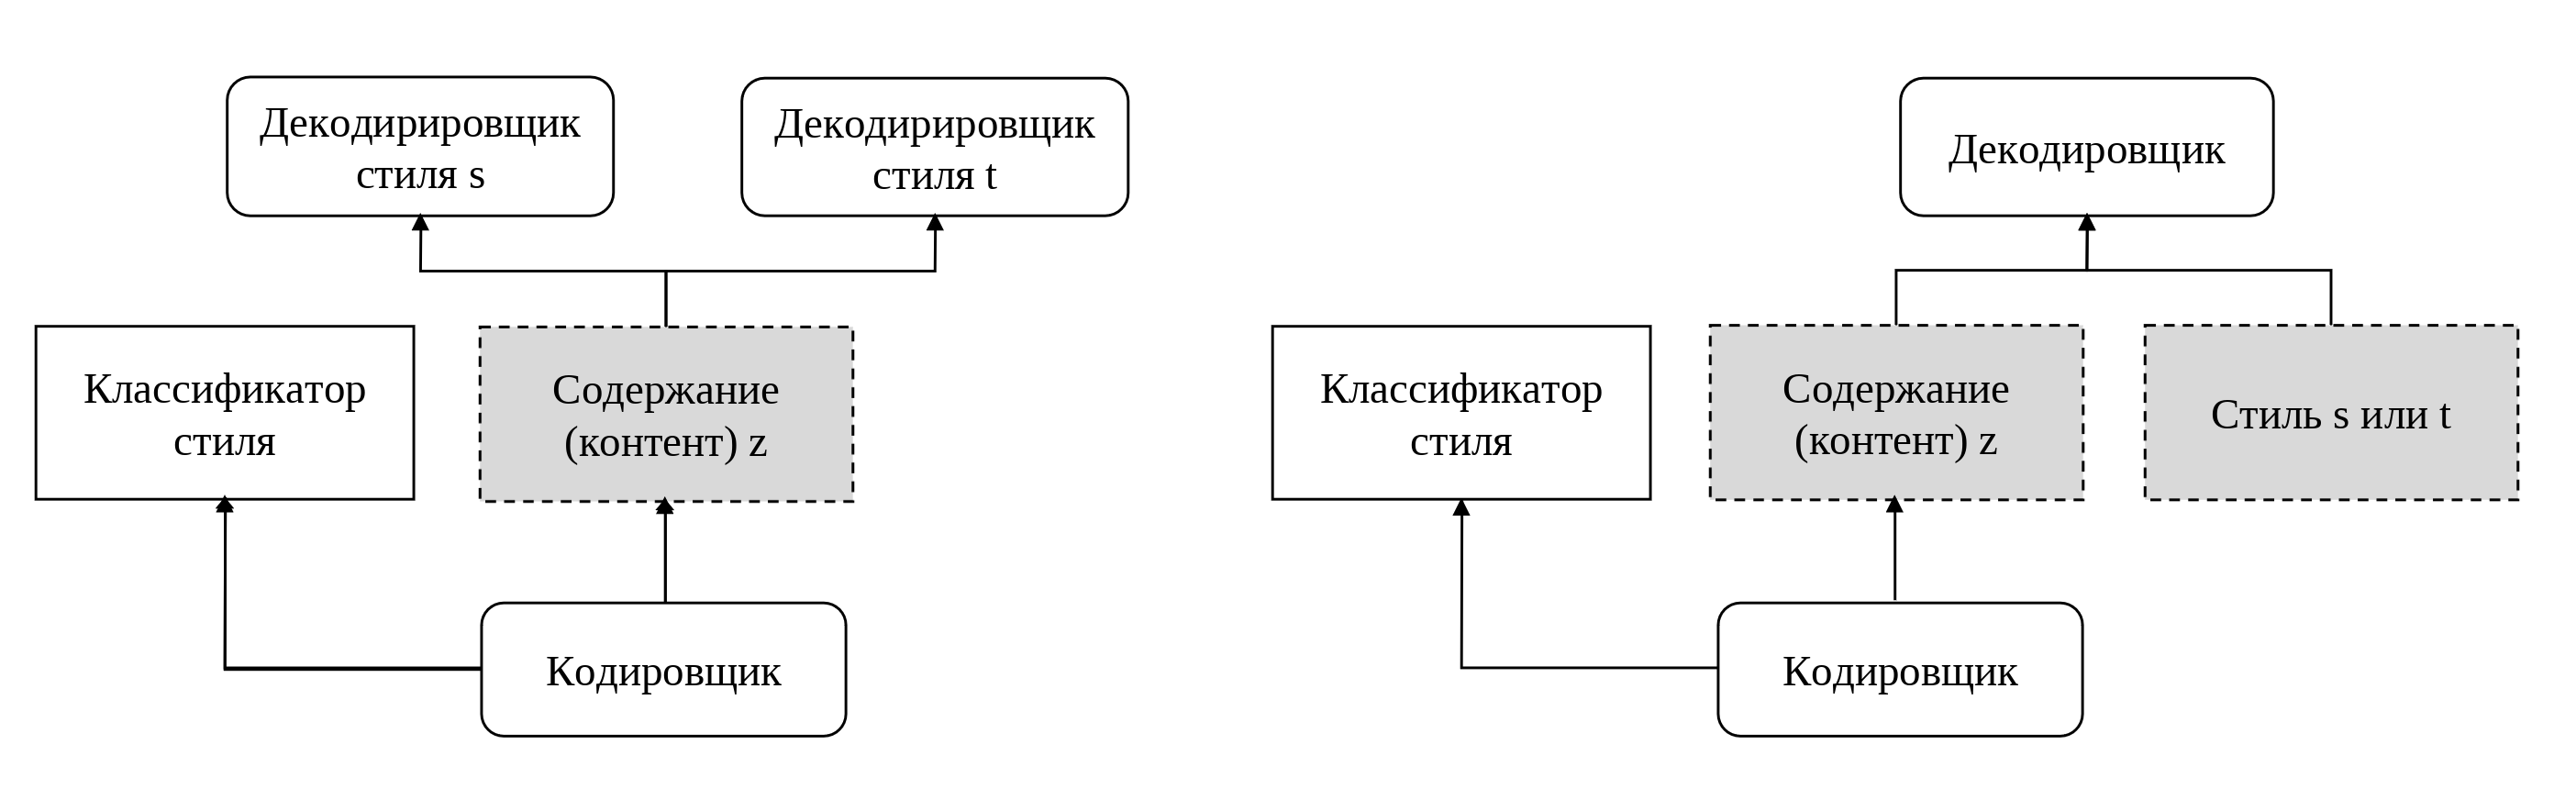
\includegraphics[width=1.0\textwidth]{figures/analysis_adversarial.png}}
  \caption{Состазательное обучение. Слева: подход с использованием нескольких декодировщиков. Справа: подход и использованием стилистических эмбеддингов}
  \label{fig:analysis_adversarial}
\end{figure}

Сама состязательная сесть состоит из двух главных компонент.
Первый компонент (дискриминатор) предназначен для классификации стиля входной последовательности $x$ на основе его латентного представления, созданного кодировщиком.
Функция потерь, которую необходимо минимизировать, -- это отрицательная логарифмическая вероятность меток стилей в обучающих данных:
$$
L_{adv1}(\Theta_D) =
- \sum_{i=1}^{M} \log p (l_i | \text{Encoder}(x_i; \Theta_E); \Theta_D)
$$
где $\Theta_D$ и $\Theta_E$ это параметры дискриминатора и кодировщика соответственно.  $M$ обозначает размер обучающего набора данных, а $l_i$ обозначает метку стиля.

Второй компонент предназначен для обмана дискриминатора, чтобы тот не мог правильно идентифицировать стиль входной последовательности $x$.
В этом случае функция потерь представляет собой максимизацию энтропии предсказаных меток стиля:
$$
L_{adv2}(\Theta_E) =
- \sum_{i=1}^M \sum_{j=1}^N
H(p(j|\text{Encoder}(x_i; \Theta_E); \Theta_D))
$$
где $N$ - количество стилей.
Обе части состязательной сети обновляют различный набор параметров.
Они работают вместе, чтобы гарантировать, что выход $\text{Encoder}(x_i;\Theta_E)$ не содержит стилистическую информацию.

Как только кодировщик обучен создавать латентное представление, два генеративных подхода генерируют текст в целевом стиле.
Первый подход подразумевает обучение нескольких декодеров под каждый стиль.
Второй подход использует обучение стилистических эмбеддингов и конкатенации их с представлением содержимого для генерации текста в целевом стиле с помощью декодера.

\subsection{Построение параллельного псевдо-корпуса}
\label{cha:analysis:subsection:backtranslation}
Обратный перевод (Back-Translation) изначально использовался в задаче машинного перевода для создания искуственного обучающего корпуса \cite{sennrich2016improving}.
Затем данный подход был успешно использован в задачах переноса стиля.
Выделяют два основных способа, основанных на поиске и генерации данных.

Первым из способов построения псевдопараллельных данных является поиск, а именно извлечение выровненных пар предложений из двух непараллельных корпусов в разных стилях.
В \textit{Unsupervised text attribute transfer via iterative matching and translation} \cite{jin2020imat} эмпирически показано, что семантически сходные предложения в двух стилистически разных корпусах, как правило, являются аналогами друг друга, отличающимися атрибутами стиля.
Следовательно, в работе строят изначальный псевдо-корпус путем сопоставления пар предложений в соответствии с косинусным сходством предварительно обученных эмбеддингов предложений.
Для каждого предложения $x$, его псевдо-аналог $\widehat{x'}$ это самое похожее предложение в другом корпусе $X'$:
$$
\widehat{x'} = \arg \max_{x' \in X'} \text{Similarity}(x, x')
$$

Второй способ является генеративным, такой как итеративный обратный перевод (Iterative Back-Translation, IBT) в работе \textit{Iterative back-translation for neural machine translation} \cite{hoang-etal-2018-iterative}.
Прежде чем начать итеративный процесс IBT должен инициализировать две модели преноса стиля: $M_{a \rightarrow a'}$, переводящая из стиля $a$ в стиль $a'$, и $M_{a' \rightarrow a}$, делающая обратное.
Затем на каждой итерации выполняется следующая последовательность шагов:
\begin{enumerate}
    \item Используются имеющиеся модели для генерации псевдо-параллельного корпуса.
    $M_{a \rightarrow a'}(x)$ генерирует псведо-пары $(x, \widehat{x'})$ для $\forall x \in X$,
    а $M_{a' \rightarrow a}(x)$ генерирует $(\widehat{x}, x')$ для $\forall x' \in X'$;
    \item Повторно обучаются эти две модели переноса стиля на наборах данных, сгенерированных на первом шаге.
    То есть обучаются $M_{a \rightarrow a'}(x)$ на парах $(\widehat{x}, x')$,
    а $M_{a' \rightarrow a}(x)$ на $(x, \widehat{x'})$.
\end{enumerate}

% На самом первом шаге простым вариантом инициализации является случайная инициализация двух моделей $M_{a \rightarrow a'}$ и $M_{a' \rightarrow a}$.
% Однако, так как этот способ подвержен случайности, обучение модели может не сойтись.




\subsection{Генерация с помощью управления атрибутами}
Этот метод подразумевает использование кода атрибута $a$ для управления генерацией текста в различных стилях.
% Существуют две стратегии генерации c помощью управления атрибутами:
% \begin{enumerate}
%     \item неявное ограничение латентного пространства $z$, чтобы оно содержало только информацию о содержимом, при изучении кода атрибута стиля;
%     \item без ограничения латентного пространства $z$ на содержание только информации о содержимом, при изучении кода атрибута стиля.
% \end{enumerate}

% В обоих стратегиях 
Функция потерь, управляемая классификатором, используется для гарантии того, что генератор $G$ сгенерирует предложение $x'$ с требуемым
атрибутом стиля.
А именно, функция потерь минимизирует:
$$
L_{cls}(\Theta_G, t) = -\mathbb{E}_{p(x)} [\log D(x')]
$$
где $D$ это классификатор стиля (дискриминатор), обученный на данных $x$.

Так как метод генерации с помощью управления атрибутами сильно зависит от классификатора стиля, этот подход имеет такие же недостатки, как и методы состязательного обучения.
В частности, точность классификатора стилей ограничивает выучивание качественных стилистических атрибутов.

В работе \textit{Toward controlled generation of text} \cite{hu2018controlled} используется вариационный автокодировщик (variational auto-encoder, VAE) \cite{kingma2022autoencoding}, который выучивает латентное пространство $z$, и классификатор стиля, чтобы выучить векто стилистических атрибутов $a$.
% Работа \textit{Toward controlled generation of text} \cite{hu2018controlled} является ярким представителем первой стратегии (неявное ограничение латентого пространства) и проиллюстрирована на рисунке \ref{fig:analysis_controled_text_generation}.
% Предлагаемая модель использует вариационный автокодировщик (variational auto-encoder, VAE) \cite{kingma2022autoencoding}, который выучивает латентное пространство $z$, и классификатор стиля, чтобы выучить векто стилистических атрибутов $a$.
Для этого используется следующая функция потерь:
$$
L_{VAE}(\Theta_G, \Theta_E; x) = 
KL(q_E(z|x) || p(z))
- E_{q_E(z|x)q_D(a|x)} [\log p_G (x| z,a)]
$$
где $KL(\cdot||\cdot)$ это дивергенция Кульбака-Лейблера, $\Theta_E$ и $\Theta_G$ -- параметры энкодера и декодера соответственно.
Условный вероятностный кодировщик $E$, обозначаемый как $q_E(z|x)$, выводит латентное представление $z$ по заданному входному предложению $x$.
$q_D(a|x)$ -- это условное распределение, определенное классификатором $D$ для каждой структурированной переменной в $a$. 
Общая схема модели проиллюстрирована на рисунке \ref{fig:analysis_controled_text_generation}.

Чтобы гарантировать, что $z$ сохраняет только информацию о семантике, не зависящую от стиля, предлагается ограничение независимости, гарантирующее, что латентное представление $z$ входного предложения $x$ и переданное предложение стиля $x'$ остаются близкими друг к другу.
Добавленное ограничение независимости, по существу, гарантирует, что информация о содержимом отделена от входного текста и закодирована в латентном представлении $z$.

\begin{figure}[ht]
  \centering
  \frame{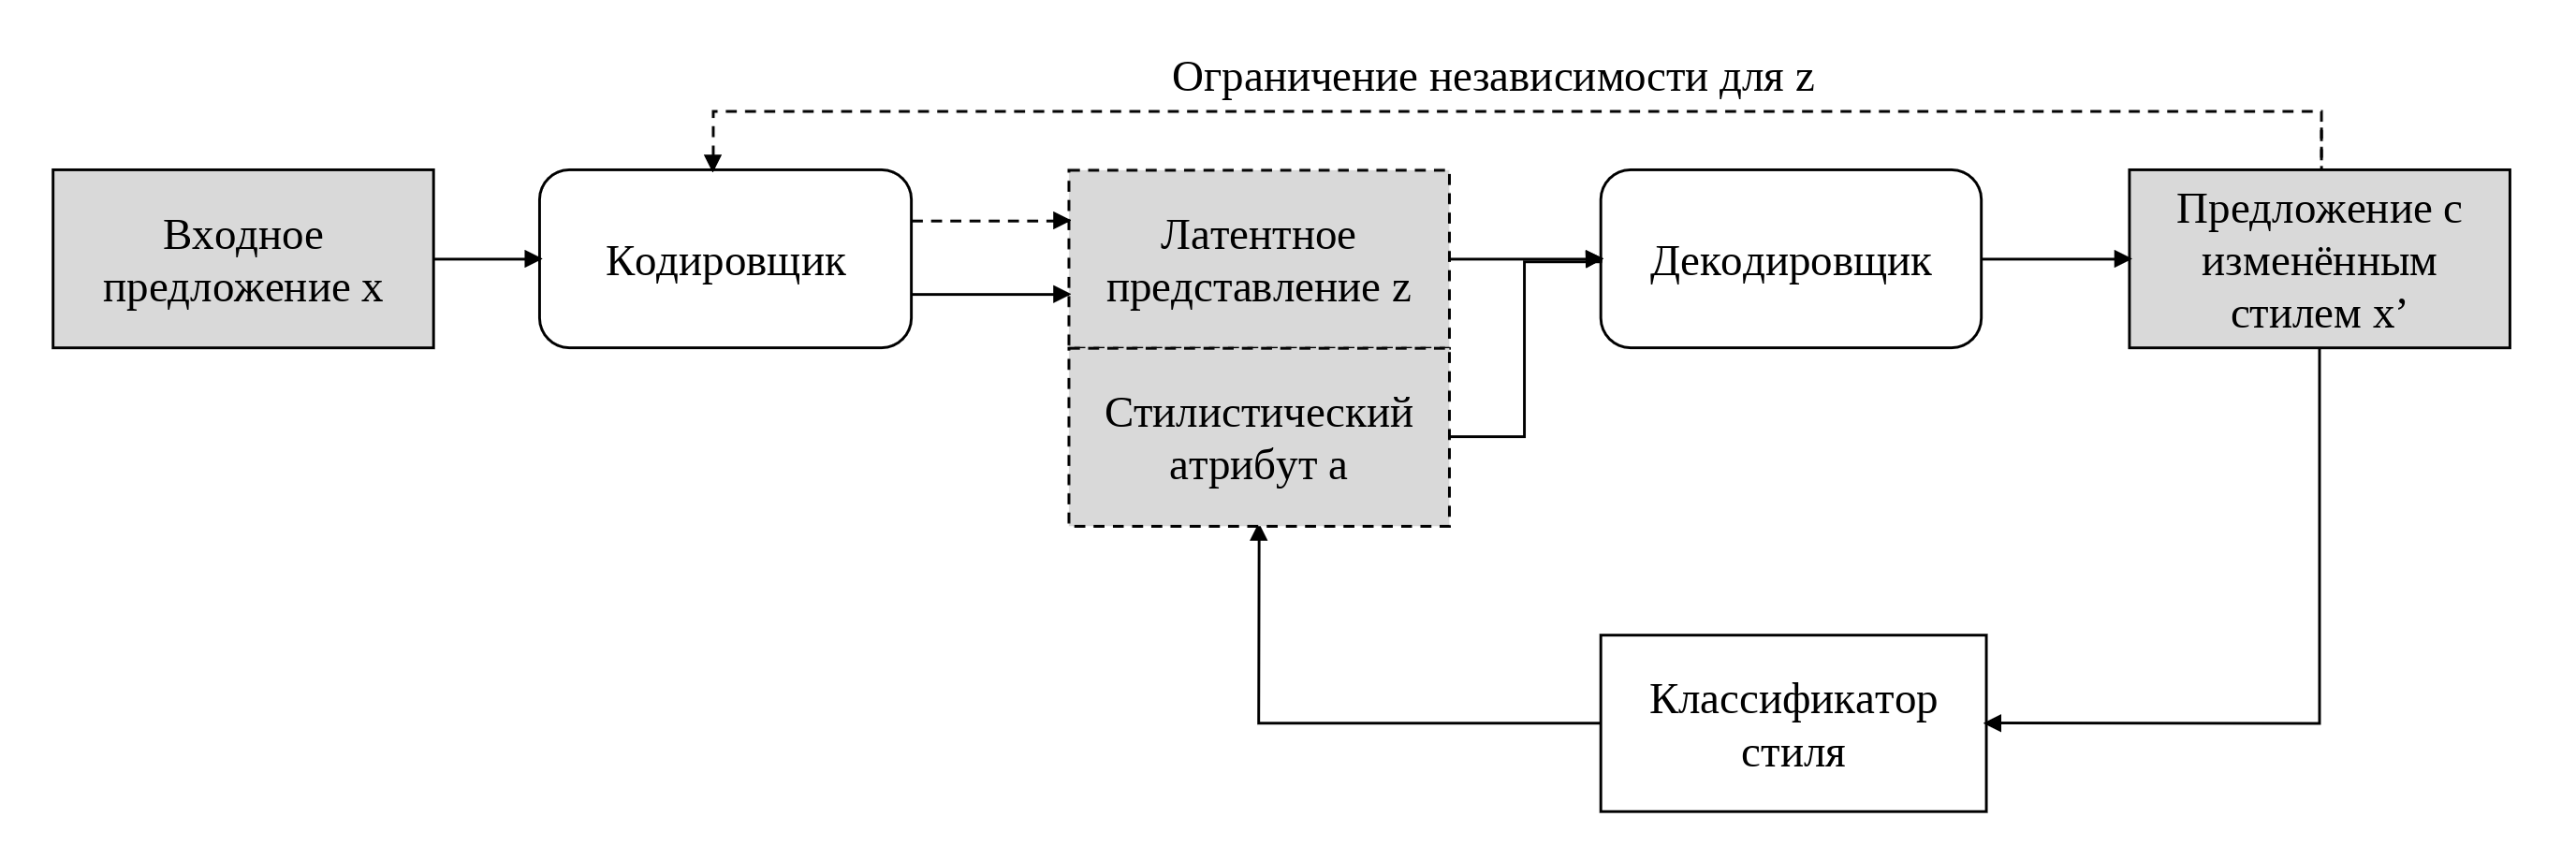
\includegraphics[width=1.0\textwidth]{figures/analysis_controled_text_generation.png}}
  \caption{Использование VAE для редактирования латентного пространства для трансфера стиля текста}
  \label{fig:analysis_controled_text_generation}
\end{figure}

% В работе \textit{Multiple-attribute text rewriting} \cite{subramanian2019multipleattribute} утверждалось, что задача разделения содержания и стиля в тексте является сложной.
% Поэтому, были предложены методы без этого.
% На рисунке \ref{fig:analysis_lample} проиллюстрированна модель, предложенная в этой работе.
% Модель использует варационный автокодировщик и механизм back-translation \ref{cha:analysis:subsection:backtranslation}.
% Сначала функция зашумления 

% \begin{figure}[ht]
%   \centering
%   \frame{\includegraphics[width=1.0\textwidth]{figures/analysis_lample.png}}
%   \caption{Генерация с помощью управления атрибутами с back-translation}
%   \label{fig:analysis_lample}
% \end{figure}

% ================================================================================
\subsection{Манипуляции в латентном пространстве}
Другим подходом к решению задачи переноса стиля текста является внесение изменений в латентное пространство, полученное от обучения модели автокодировщика.
%QUESTION: нужен тут риснок?
Рисунок \ref{fig:analysis_latent_repr_editing} иллюстрирует этот метод.
\begin{figure}[ht]
  \centering
  \frame{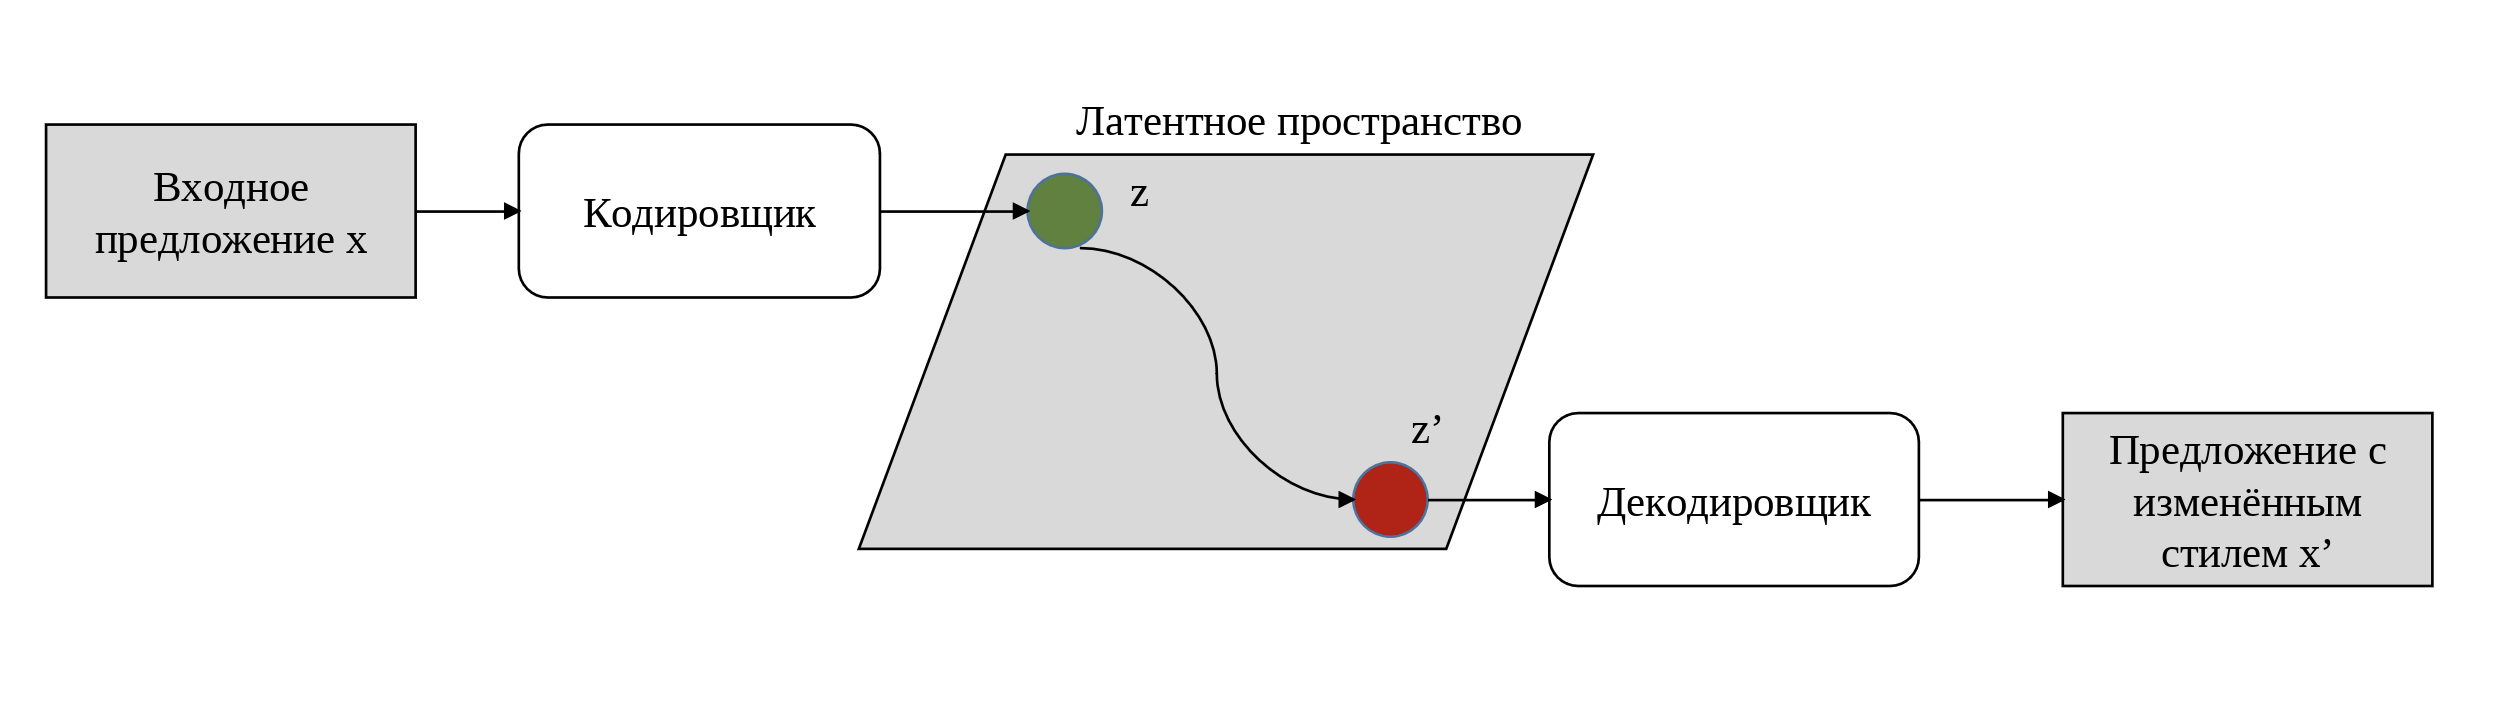
\includegraphics[width=1.0\textwidth]{figures/analysis_latent_repr_editing.png}}
  \caption{Общая структура редактирования латентного пространства для трансфера стиля текста}
  \label{fig:analysis_latent_repr_editing}
\end{figure}

% QUESTION автоэнкодер можно сказать?
Классификатор стиля обучается совместно с автоэнкодером.
Во время обучения итеративно обновляется латентное пространство $z$ в ограниченном пространстве, чтобы максимизировать точность классификатора.
А именно, каждое обновление вычисляется на основе градиента потери классификатора стилей относительно $z$.
Обработанное латентное представление $z'$ затем подаётся в декодер для генерации текста целевого стиля.

Главной проблемой методов этого семейства является определение границ, в пределах которых должна происходить манипуляция в латентном пространстве.
Было замечено, что декодер не может генерировать предложения в целевом стиле, если полученное после редактирования латентного пространства выходит за пределы областей представления, увиденных декодером во время обучения \cite{mueller_seq2betterseq}.
Существующие решения направлены на ограничение манипуляций в рамках ограниченного латентного пространства.


% ================================================================================
\subsection{Обучение с подкреплением}
Ключевая идея алгоритмов, основанных на обучении с подкреплением, это использование специально разработанных функций вознаграждения для управления процессом переноса стиля вместо различных функций потерь, используемых в
другим методах.

Алгоритм \textit{Policy Gradient} \cite{Williams1992SimpleSG} используется для максимизации ожидаемого вознаграждения за перефразированный текст.
% Алгоритм Policy Gradient упрощает обучение, не беспокоясь о сложности дискретного обучения, вызванной процессом автоматического регрессионного декодирования.
Однако из-за высокой дисперсии градиента выборки обучение с помощью этого метода может быть нестабильным.

В работе \textit{A Dual Reinforcement Learning Framework for Unsupervised Text Style Transfer} \cite{luo2019dual} предложено обучать две Seq2Seq модели между двумя стилями посредством обучения с подкреплением, не разделяя стиль и семантику.
Авторы рассматривали обучение модели переноса стиля из исходного в целевой и из целевого в обратный как двойную задачу.
Награда за классификатор стилей $R_S$ и награда за реконструкцию $R_C$ предназначены для повышения точности передачи стиля и сохранения семантики.
Общая награда является гармоническим средним из двух вознаграждений, и она использовалась в качестве сигнала обратной связи для обучения в
структуре с двумя задачами.
Таким образом, модель может быть обучена с помощью обучения с подкреплением без параллельных данных. Общая схема обучения представлена на рисунке \ref{fig:analysis_rl}
% QUESTION по термину "двойной" не уверен
% QUESTION нужна тут вообще картинка?
\begin{figure}[ht]
  \centering
  \frame{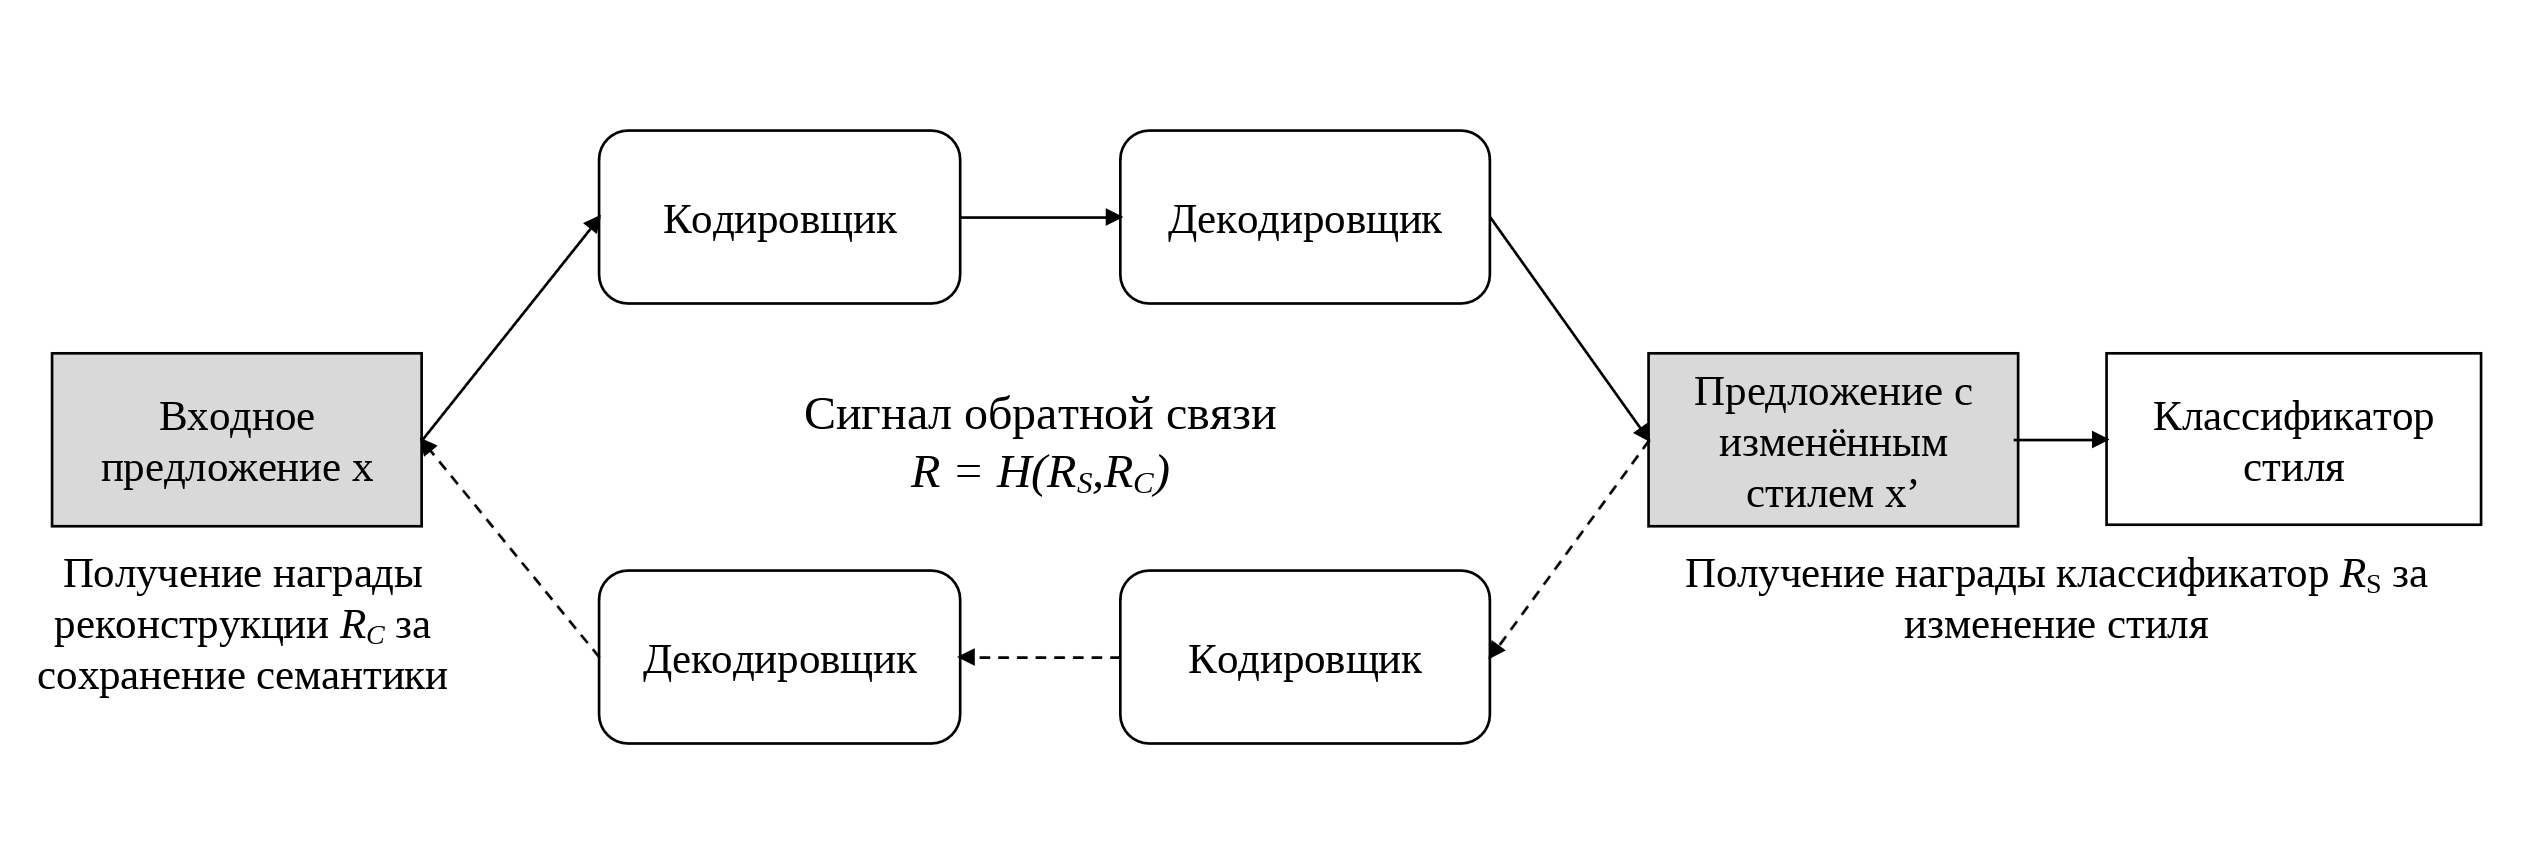
\includegraphics[width=1.0\textwidth]{figures/analysis_rl.png}}
  \caption{Модель двойного обучения с подкреплением}
  \label{fig:analysis_rl}
\end{figure}

Хотя существующие методы обучения с подкреплением по-прежнему в значительной степени опираются на классификаторы стилей для управления процессом переноса стиля, этот подход дает возможность разработать другие функции вознаграждения, которые будут направлять процесс переноса стиля.

